
\begin{figure}[t]
  \begin{center}
    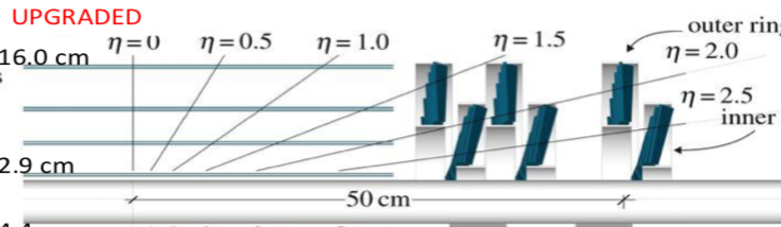
\includegraphics[width=0.9\linewidth]{plots/PixLayout.png}
    \caption{
      Layout of the Run II Pixel detector showing the 4 Barrel layers (0,1,2,3) and 3 Forward disks composed of 2 Panels each. 
    \label{fig:pixellayout}
    }
  \end{center}
\end{figure}


The layout of one quadrant of the Pixel detector used in CMS for  Run II is shown in Fig~\ref{fig:pixellayout}.
It is composed of a Barrel section with 4 layers and the Forward section with 3 disks (each with 2 Panels).
The Pixel sensors are read out by a total of 1856 modules.
A stability study comparing different periods in 2018 was used to exclude a list of modules which showed large variations between periods.
From this study a total of 1387 modules are removed, this veto list can be found in Appendix~\ref{sec:appendix1} and maps per detector section are shown in figure~\ref{fig:pixelmodvetomap} and table~\ref{tab:pixveto}.


\begin{table}[hc]
\caption{Number of vetoed modules per Pixel section.}
\label{tab:pixveto}
\begin{center}
\begin{tabular}{l|c|c}
\hline
\multirow{2}{*}{Section} & \multicolumn{2}{c}{$\#$ of Removed modules}  \\
  & $-$Side & $+$Side \\
\hline
BPIX layer 0 & - & - \\
BPIX layer 1 & 108 & 110 \\
BPIX layer 2 & 94  & 168 \\
BPIX layer 3 & 111 & 186 \\
FPIX Panel 0 & 122 & 122 \\
FPIX Panel 1 & 140 & 132 \\
\hline\hline
\end{tabular}
\end{center}
\end{table}


\newpage
\begin{figure}[hc]
  \begin{center}
    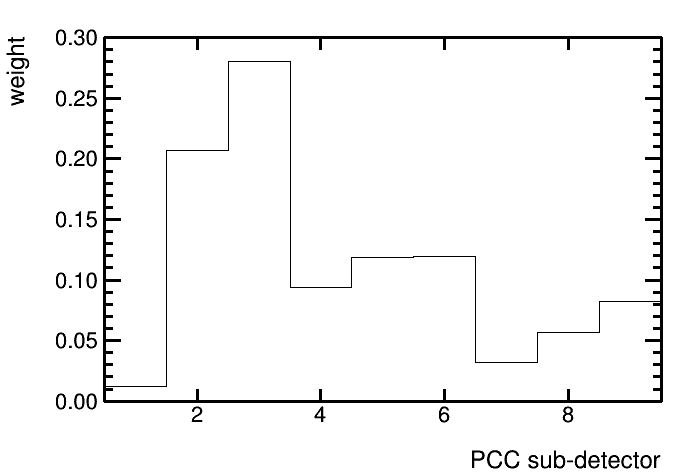
\includegraphics[width=0.7\linewidth]{plots/PCCWeights.png}
    \caption{
      Fraction of total clusters per each part of the Pixel detector. The weights are determined after applying the module veto list.
      Bins 1,2,3 correspond to the BPIX layers, bins 4,5,6 correspond to the FPIX Panel 0 disks (inner), and 7,8,9 to the FPIX Panel 1 disks (outer).
      \label{fig:pixelweights}
    }
  \end{center}
\end{figure}



\newpage
\begin{figure}[hbt]
  \begin{center}

    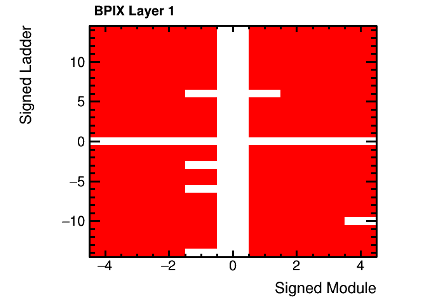
\includegraphics[width=0.45\linewidth]{plots/VetoMap_BPIX1.png}\\
    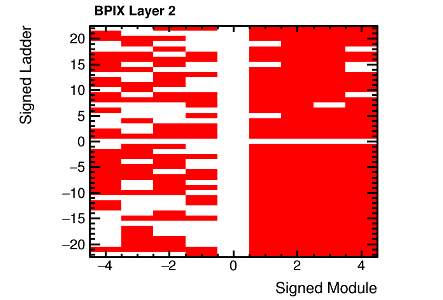
\includegraphics[width=0.45\linewidth]{plots/VetoMap_BPIX2.png}
    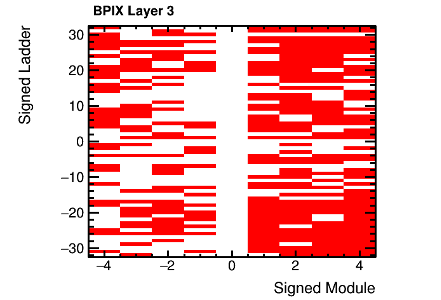
\includegraphics[width=0.45\linewidth]{plots/VetoMap_BPIX3.png}
    \vspace{20pt}
    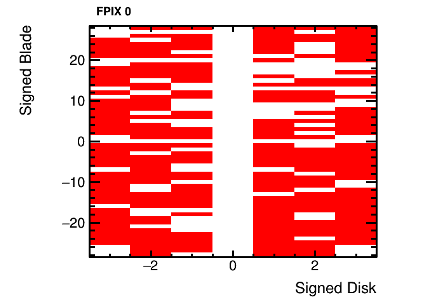
\includegraphics[width=0.45\linewidth]{plots/VetoMap_FPIX0.png}
    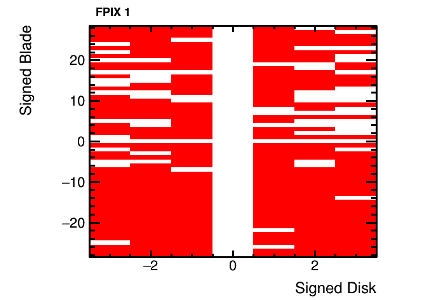
\includegraphics[width=0.45\linewidth]{plots/VetoMap_FPIX1.png}
    \caption{
      Maps of Pixel modules vetoed in the PCC luminosity computation. The veto list corresponds to the study performed using 2018 data including Run D period.
    \label{fig:pixelmodvetomap}
    }
  \end{center}
\end{figure}
